\documentclass[border=15pt, multi, tikz]{standalone}
\usepackage{import}
\usepackage{etoolbox}
\usepackage{graphicx}
\usepackage{svg}
\usepackage{colortbl}

\usetikzlibrary{positioning,matrix,fit}
\usetikzlibrary{3d} %for including external image
\usetikzlibrary{decorations,shapes}
\usetikzlibrary{decorations.shapes}
\usetikzlibrary{decorations.markings}
\usetikzlibrary{decorations.pathreplacing}
\usetikzlibrary{backgrounds}
\usetikzlibrary{calc}
\usetikzlibrary{arrows.meta,arrows}
\graphicspath{{image/}}


\usepackage{bm}
\usepackage{relsize}
\usepackage{pgfplots}


\tikzset{%
  % Specifications for style of nodes:
    zoom/.style = {densely dotted, very thick,opacity=.3},
    lstmCell/.style = {rectangle, rounded corners=10, minimum width=5em, minimum height=3em, draw, very thick},
    stealthArrow/.style={-stealth, very thick},
    stealthArrowW/.style={-stealth, line width=1mm, white},
}
 
\usetikzlibrary{decorations.pathmorphing}

\begin{document}
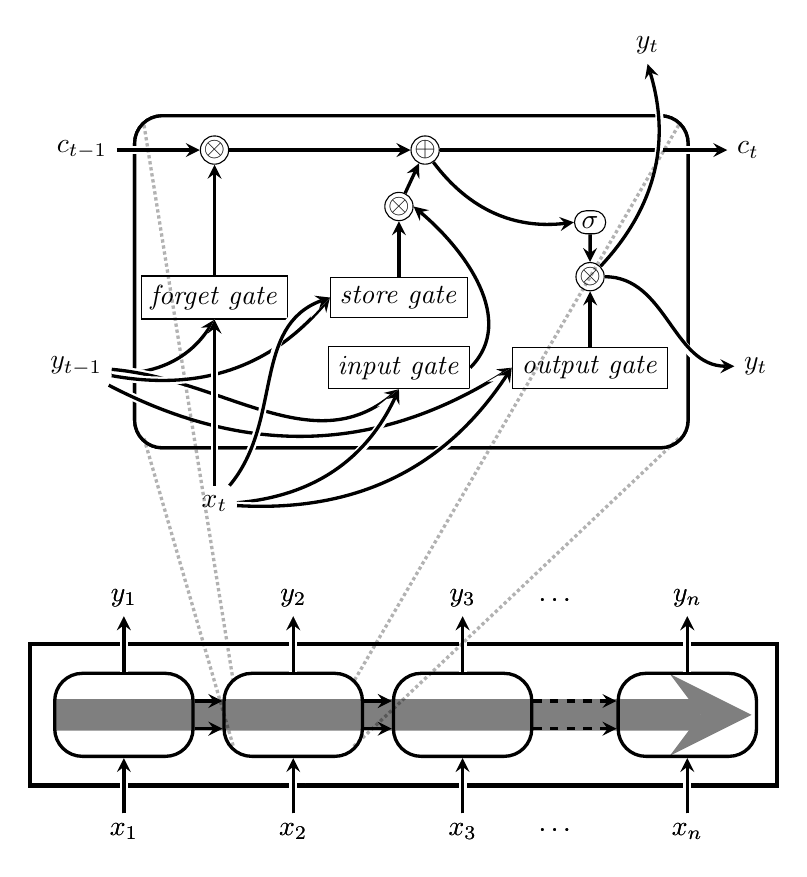
\begin{tikzpicture}
	\node[rectangle, rounded corners=10, minimum width=20em, minimum height=12em, draw, very thick] (lstm) at (0, 0) {};
	
	
	\node[lstmCell] (lst2) at (-1.5, -5.5) {};
	
	\node[lstmCell,left=1em of lst2] (lst1) {};
	
	\node[lstmCell,right=1em of lst2] (lst3) {};
	
	\node[right=0.5em of lst3] (dots) {};
	
	\node[lstmCell,right=3em of lst3] (lst4) {};
	
	\node[rectangle, minimum width=27em, minimum height=5.1em, ultra thick, draw] at (-0.1, -5.5) (chn1) {};
	\begin{scope}[transparency group, opacity=0.5]
	\draw[-stealth, line width=4mm] ([xshift=+1em]chn1.west) -- ([xshift=-1em]chn1.east);
	\end{scope}
	
	\node[below=2em of lst1] (x1) {$x_1$};
	\node[below=2em of lst2] (x2) {$x_2$};
	\node[below=2em of lst3] (x3) {$x_3$};
	\node[below=3.4em of dots] (xd) {\dots};
	\node[below=2em of lst4] (x4) {$x_n$};
	\node[above=2em of lst1] (y1) {$y_1$};
	\node[above=2em of lst2] (y2) {$y_2$};
	\node[above=2em of lst3] (y3) {$y_3$};
	\node[above=3.4em of dots] (yd) {\dots};
	\node[above=2em of lst4] (y4) {$y_n$};
	
	\draw[-stealth, line width=1mm, white] (x1) -- (lst1);
	\draw[-stealth, line width=1mm, white] (x2) -- (lst2);
	\draw[-stealth, line width=1mm, white] (x3) -- (lst3);
	\draw[-stealth, line width=1mm, white] (x4) -- (lst4);
	\draw[-stealth, very thick] (x1) -- (lst1);
	\draw[-stealth, very thick] (x2) -- (lst2);
	\draw[-stealth, very thick] (x3) -- (lst3);
	\draw[-stealth, very thick] (x4) -- (lst4);
	
	\draw[-stealth, line width=1mm, white] (lst1) -- (y1);
	\draw[-stealth, line width=1mm, white] (lst2) -- (y2);
	\draw[-stealth, line width=1mm, white] (lst3) -- (y3);
	\draw[-stealth, line width=1mm, white] (lst4) -- (y4);
	\draw[-stealth, very thick] (lst1) -- (y1);
	\draw[-stealth, very thick] (lst2) -- (y2);
	\draw[-stealth, very thick] (lst3) -- (y3);
	\draw[-stealth, very thick] (lst4) -- (y4);
	
	\draw[-stealth, very thick] ([yshift=-0.5em]lst1.east) -- ([yshift=-0.5em]lst2.west);
	\draw[-stealth, very thick] ([yshift=+0.5em]lst1.east) -- ([yshift=+0.5em]lst2.west);
	\draw[-stealth, very thick] ([yshift=-0.5em]lst2.east) -- ([yshift=-0.5em]lst3.west);
	\draw[-stealth, very thick] ([yshift=+0.5em]lst2.east) -- ([yshift=+0.5em]lst3.west);
	\draw[-stealth, dashed, very thick] ([yshift=-0.5em]lst3.east) -- ([yshift=-0.5em]lst4.west);
	\draw[-stealth, dashed, very thick] ([yshift=+0.5em]lst3.east) -- ([yshift=+0.5em]lst4.west);

	\node[rectangle, minimum width=27em, minimum height=5.1em, ultra thick, draw, fill=white] at (-0.1, -5.5) (chn1) {};
	

	
	\node[rectangle, rounded corners=10, minimum width=20em, minimum height=12em, draw, very thick, fill=white] (lstm) at (0, 0) {};
	
	\node[rectangle, draw] at (-2.5, -.2) (FG1) {\emph{forget gate}};
	\node[rectangle, draw, right=1.5em of FG1] (SG1) {\emph{store gate}};
	\node[rectangle, draw, below=1em of SG1] (IG1) {\emph{input gate}};
	\node[rectangle, draw, right=1.5em of IG1] (OG1) {\emph{output gate}};
	\node[circle, draw, above=2em of SG1, inner sep=0em] (m1) {$\otimes$};
	\node[circle, draw, above=4em of FG1, inner sep=0em] (m2) {$\otimes$};
	\node[circle, draw, right=6.55em of m2, inner sep=0em] (p1) {$\oplus$};
	\node[circle, draw, above=2em of OG1, inner sep=0em] (m3) {$\otimes$};
	\node[rounded rectangle, draw, above=1em of m3, inner sep=0.2em] (tt) {$\sigma$};
	
	\node[below=6em of FG1] (xt) {$x_t$};
	\node[below=1em of FG1, xshift=-5em] (ht1) {$y_{t-1}$};
	\node[left=3em of m2] (ct1) {$c_{t-1}$};
	\node[right=18em of m2] (ct) {$c_t$};
	\node[right=22.5em of ht1] (ht) {$y_t$};
	\node[] (yt) at (3, 3) {$y_t$};
	
		
	% y_{t-1} input to gates
	\draw[stealthArrowW, bend right] (ht1) to (FG1.south);
	\draw[stealthArrow, bend right] (ht1) to (FG1.south);
	\path[stealthArrowW] (ht1) edge[out=355,in=220] (IG1.south);
	\path[stealthArrow] (ht1) edge[out=355,in=220] (IG1.south);
	\path[stealthArrowW] (ht1) edge[bend right] (SG1.west);
	\path[stealthArrow] (ht1) edge[bend right] (SG1.west);
	\path[stealthArrowW] (ht1) edge[bend right] (OG1.west);
	\path[stealthArrow] (ht1) edge[bend right] (OG1.west);
	
	% x_t input to gates
	\draw[stealthArrowW] (xt) -- (FG1);
	\draw[stealthArrow] (xt) -- (FG1);
	\path[stealthArrowW] (xt) edge[bend right] (IG1.south);
	\path[stealthArrow] (xt) edge[bend right] (IG1.south);
	\draw[stealthArrowW,out=50,in=200] (xt) to (SG1.west);
	\draw[stealthArrow,out=50,in=200] (xt) to (SG1.west);
	\path[stealthArrowW] (xt) edge[bend right] (OG1.west);
	\path[stealthArrow] (xt) edge[bend right] (OG1.west);
	

	
	
	\draw[-stealth, very thick] (FG1) -- node[left] {} (m2);
	\draw[-stealth, very thick, out=45, in=320] (IG1.east) to (m1.east);
	\draw[-stealth, very thick] (SG1) -- node[right] {} (m1);
	\draw[-stealth, very thick] (m1) -- (p1);
	\draw[-stealth, line width=1mm, white] (ct1) -- (m2);
	\draw[-stealth, very thick] (ct1) -- (m2);
	\draw[-stealth, very thick] (m2) -- (p1);
	\draw[-stealth, very thick] (OG1) -- (m3);
	
	\draw[-stealth, line width=1mm, white] (p1) -- (ct);
	\draw[-stealth, very thick] (p1) -- (ct);
	\draw[-stealth, very thick] (tt) -- (m3);
	\draw[-stealth, line width=1mm, white] (m3) edge[out=0, in=180] (ht.west);
	\draw[-stealth, very thick] (m3) edge[out=0, in=180] (ht.west);
	
	\draw[-stealth ,very thick] (p1) edge[bend right] (tt.west);
	\draw[-stealth, line width=1mm,white] (m3) edge[bend right] (yt.south);
	\draw[-stealth, very thick] (m3) edge[bend right] (yt.south);
	
	\node[lstmCell] (lst2) at (-1.5, -5.5) {};
	
	\node[lstmCell,left=1em of lst2] (lst1) {};
	
	\node[lstmCell,right=1em of lst2] (lst3) {};
	
	\node[right=0.5em of lst3] (dots) {};
	
	\node[lstmCell,right=3em of lst3] (lst4) {};
	
	\begin{scope}[transparency group, opacity=0.5]
	\draw[-stealth, line width=4mm] ([xshift=+1em]chn1.west) -- ([xshift=-1em]chn1.east);
	\end{scope}
	
	\node[below=2em of lst1] (x1) {$x_1$};
	\node[below=2em of lst2] (x2) {$x_2$};
	\node[below=2em of lst3] (x3) {$x_3$};
	\node[below=3.4em of dots] (xd) {\dots};
	\node[below=2em of lst4] (x4) {$x_n$};
	\node[above=2em of lst1] (y1) {$y_1$};
	\node[above=2em of lst2] (y2) {$y_2$};
	\node[above=2em of lst3] (y3) {$y_3$};
	\node[above=3.4em of dots] (yd) {\dots};
	\node[above=2em of lst4] (y4) {$y_n$};
	
	\draw[-stealth, line width=1mm, white] (x1) -- (lst1);
	\draw[-stealth, line width=1mm, white] (x2) -- (lst2);
	\draw[-stealth, line width=1mm, white] (x3) -- (lst3);
	\draw[-stealth, line width=1mm, white] (x4) -- (lst4);
	\draw[-stealth, very thick] (x1) -- (lst1);
	\draw[-stealth, very thick] (x2) -- (lst2);
	\draw[-stealth, very thick] (x3) -- (lst3);
	\draw[-stealth, very thick] (x4) -- (lst4);
	
	\draw[-stealth, line width=1mm, white] (lst1) -- (y1);
	\draw[-stealth, line width=1mm, white] (lst2) -- (y2);
	\draw[-stealth, line width=1mm, white] (lst3) -- (y3);
	\draw[-stealth, line width=1mm, white] (lst4) -- (y4);
	\draw[-stealth, very thick] (lst1) -- (y1);
	\draw[-stealth, very thick] (lst2) -- (y2);
	\draw[-stealth, very thick] (lst3) -- (y3);
	\draw[-stealth, very thick] (lst4) -- (y4);
	
	\draw[-stealth, very thick] ([yshift=-0.5em]lst1.east) -- ([yshift=-0.5em]lst2.west);
	\draw[-stealth, very thick] ([yshift=+0.5em]lst1.east) -- ([yshift=+0.5em]lst2.west);
	\draw[-stealth, very thick] ([yshift=-0.5em]lst2.east) -- ([yshift=-0.5em]lst3.west);
	\draw[-stealth, very thick] ([yshift=+0.5em]lst2.east) -- ([yshift=+0.5em]lst3.west);
	\draw[-stealth, dashed, very thick] ([yshift=-0.5em]lst3.east) -- ([yshift=-0.5em]lst4.west);
	\draw[-stealth, dashed, very thick] ([yshift=+0.5em]lst3.east) -- ([yshift=+0.5em]lst4.west);
	
	
	% dotted lines from big cell to the small one
	\draw[zoom] ([xshift=0.4em,yshift=-0.4em]lstm.north west) -- ([xshift=0.4em,yshift=-0.4em]lst2.north west);
	\draw[zoom] ([xshift=-0.4em,yshift=-0.4em]lstm.north east) -- ([xshift=-0.4em,yshift=-0.4em]lst2.north east);
	\draw[zoom] ([xshift=-0.4em,yshift=0.4em]lstm.south east) -- ([xshift=-0.4em,yshift=0.4em]lst2.south east);
	\draw[zoom] ([xshift=0.4em,yshift=0.4em]lstm.south west) -- ([xshift=0.4em,yshift=0.4em]lst2.south west);
	
\end{tikzpicture}
\end{document}